\documentclass{article}

\usepackage{amsmath}
\usepackage{amssymb}
\usepackage{parskip}
\usepackage{fullpage}
\usepackage{hyperref}
\usepackage{gensymb}
\usepackage{tikz}

\hypersetup{
    colorlinks=true,
    linkcolor=black,
    urlcolor=blue,
    pdftitle={Thermodynamics},
    pdfpagemode=FullScreen,
}

\newcommand{\cel}{C\degree}

\title{Thermodynamics}
\author{Paolo Bettelini}
\date{}

\begin{document}

\maketitle
\tableofcontents
\pagebreak


\section{Termodinamica}

La \textbf{temperatura} è una grandezza operativa (\cel, K)
mentre il \textbf{calore} è una forma di energia (Joule).

Tipi di termometro: \textit{dilatazione} (es. mercurio),
\textit{contatto} (tensione in funzione della temperatura),
\textit{infrarossi} (potenza onda infrarossi riflessa).

La pressione di vari gas confinati è linearmente proporzionale alla temperatura.
Tutte le funzioni linear della pressione \(P(T)\) hanno lo stesso punto in comune;
quando la temperatura è \(0\) (zero assoluto).

\section{Dilatazione}

\subsection{Solidi}

La dilatazione di un oggetto in una direzione \(\Delta l\) in funzione del
cambio di temperatura \(\Delta T\) è proporzionale e data da
\[
    \Delta l = l_0 \cdot \alpha \cdot \Delta T
\]
dove \(l_0\) è la lunghezza iniziale e \(\alpha\) è il coefficiente di dilatazione lineare
\((\frac{1}{K})\). Questo funziona solamente per certi intervalli di temperatura,
ossia il solido non deve cambiare stato.

Un solido si dilata in tutte le direzioni.
La dilatazione dell'area o del volume di un solito possono essere \textit{approssimate}
nella seguente maniera
\begin{align*}
    \Delta A &\approx 2 \cdot A_0 \cdot \alpha \cdot \Delta T \\
    \Delta V &\approx 3 \cdot V_0 \cdot \alpha \cdot \Delta T
\end{align*}

\subsection{Fluidi (liquidi e gas)}

Un liquido/gas, non avendo forma propria, ha una dilatazione che può essere
quantificata solo in termini volumetrici
\[
    \Delta V = V_0 \cdot \gamma \cdot \Delta T
\]
dove \(\gamma\) è il coefficiente di dilatazione cubica.

\section{Gas}

\subsection{Trasformazione isobarica}

\begin{minipage}[left]{0.25\textwidth}
    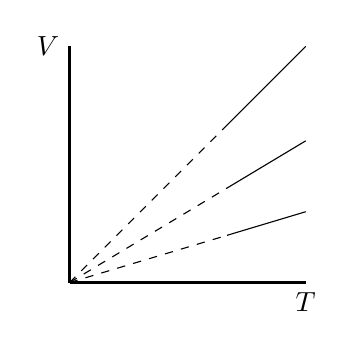
\begin{tikzpicture}
        \draw[-, thick] (0,0) -- (3,0) node[below] {\(T\)};
        \draw[-, thick] (0,0) -- (0,3) node[left] {\(V\)};

        \draw[-, dashed] (0,0) -- (2,0.6);
        \draw[-] (2,0.6) -- (3,0.9);

        \draw[-, dashed] (0,0) -- (2,2);
        \draw[-] (2,2) -- (3,3);

        \draw[-, dashed] (0,0) -- (2,1.2);
        \draw[-] (2,1.2) -- (3,1.8);
    \end{tikzpicture}
\end{minipage}
\begin{minipage}[left]{0.75\textwidth}
Cambiamento dello stato quando la pressione è costante.
\[
    \frac{V_1}{T_1} = \frac{V_2}{T_2}
\]
\end{minipage}

\subsection{Trasformazione isocòra}

\begin{minipage}[left]{0.25\textwidth}
    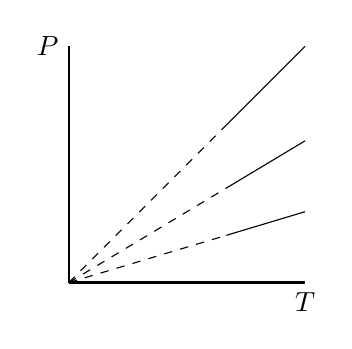
\begin{tikzpicture}
        \draw[-, thick] (0,0) -- (3,0) node[below] {\(T\)};
        \draw[-, thick] (0,0) -- (0,3) node[left] {\(P\)};

        \draw[-, dashed] (0,0) -- (2,0.6);
        \draw[-] (2,0.6) -- (3,0.9);

        \draw[-, dashed] (0,0) -- (2,2);
        \draw[-] (2,2) -- (3,3);

        \draw[-, dashed] (0,0) -- (2,1.2);
        \draw[-] (2,1.2) -- (3,1.8);
    \end{tikzpicture}
\end{minipage}
\begin{minipage}[left]{0.75\textwidth}
Cambiamento dello stato quando il volume rimane costante.
\[
    \frac{P_1}{T_1} = \frac{P_2}{T_2}
\]
\end{minipage}

\subsection{Trasformazione isotermica}

\begin{minipage}[left]{0.25\textwidth}
    \begin{tikzpicture}
        \draw[-, thick] (0,0) -- (3,0) node[below] {\(V\)};
        \draw[-, thick] (0,0) -- (0,3) node[left] {\(P\)};

        \draw[domain=0.5:2.25, smooth, variable=\x]  plot ({1 / \x}, {\x});
    \end{tikzpicture}
\end{minipage}
\begin{minipage}[left]{0.75\textwidth}
Cambiamento dello stato quando la temperatura è costante.
\[
    P_1 \cdot V_1 = P_2 \cdot V_2
\]
\end{minipage}

\subsection{Gas perfetti}

Un gas \textit{perfetto} rispetta tutte e 3 le leggi assieme
\[
    \frac{P_1 \cdot V_1}{T_1} = \frac{P_2 \cdot V_2}{T_2}
\]

\subsubsection{Equazione di stato dei gas perfetti}

Un gas perfetto rispetta l'identità
\[
    pV = nRT
\]
dove
\begin{itemize}
    \item \(p\): Pressione
    \item \(V\): Volume
    \item \(n\): Numero di moli
    \item \(R\): Costante universale dei gas \(8.314 \frac{J}{\text{mol} \cdot K}\)
    \item \(T\): Temperatura
\end{itemize}

\pagebreak

\section{Calore}

\subsection{Capacità termica}

La capacità termica di un sistema è la capacità di
cambiare temperatura scambiando calore (energia).
\[
    C=\frac{Q}{\Delta T}, \quad \left[\frac{\text{J}}{\text{K}}\right]
\]
dove \(C\) è la capacità termica.
\(Q\) è il calore scambiato e \(\Delta T\) è la variazione di temperatura.

La capacità termica di un sistema con più sostanze è data dalla somma
delle singole capacità termiche.
\[
    C_{\text{system}} = \sum_j C_j
\]

\subsection{Calore specifico}

Il calore specifico determina la capacità termica per unità di massa.
Corrisponde alla quantità di calore (energia) necessaria per innalzare,
o diminuire, di un unità la temperatura di una quantità di sostanza.
\[
    c_s = \frac{C}{m}, \quad \left[\frac{\text{J}}{\text{K}\cdot \text{Kg}}\right]
\]
dove \(c_s\) è il calore specifico. \(C\) è la capacità termica
e \(m\) è la massa.

\subsection{Calore latente}

Il calore latente è la quantità di energia per massa
durante lo svolgimento di un passaggio di stato.
\[
    L=\frac{Q}{m}, \quad \left[\frac{\text{J}}{\text{Kg}}\right]
\]


\end{document}
